\section{Klassifikation von Problemen}

Es gibt viele Arten von Problemen und sie werden durch die Informationen des L�sers bestimmt. 

\paragraph{1. Probleme mit Einfach Zust�nden}

F�r den Probleml�ser ist klar, in welchem Zustand er sich befindet und was seine m�glichen Aktionen bewirken werden. Wie bereits im Roomba-Beispiel (Kap. \ref{section:roomba}) erw�hnt, kann dies als endlicher Zustandsautomat modelliert werden.

\paragraph{2. Probleme mit Mehrfach-Zust�nden}

Der genaue Zustand, in dem sich der Probleml�ser befindet, ist nicht bekannt, und der Probleml�ser wei� nicht, was seine Aktionen bewirken werden.

Anhand des Roomba-Beispiels: In dem Extremfall dass der Roomba keine Sensoren hat, kann er als mehrfaches Problem modelliert werden. In einem solchen Fall kann der Startzustand einer der Zust�nde S1 bis S8 sein (siehe Abb. \ref{fig:roomba-simplified}).

Eine m�gliche L�sung besteht darin, die Menge der aktuell m�glichen Zust�nde zu verwenden, um die Aktionen des L�sers zu bestimmen:

\begin{figure}[H]
    \centering
    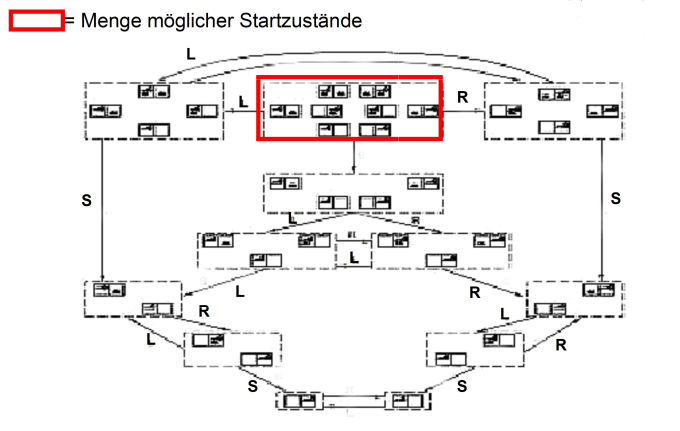
\includegraphics[width=0.8\textwidth]{figures/roomba-mehrfach.states.png}
    \caption{Staubsaugerwelt als Mehrfach-Problem}
    \label{fig:roomba-mehrfach-statemachine}
\end{figure}

\paragraph{3. Zufall-Probleme}

Der L�ser hat keine vollst�ndige Kenntnis einer sich st�ndig ver�ndernden Welt. Er kann nur die lokale Umgebung wahrnehmen.

Auch hier wieder das Roomba-Beispiel: Der Roboter befindet sich im Zustand S1 oder S3 und kann die Aktionen: Saugen, nach rechts fahren, Saugen ausf�hren. 

Der Roboter saugt und bewegt sich dann nach rechts. Wenn er aber sich vor der Bewegung im Zustand S3 befand, geht er zum Zustand S8 �ber. Er versucht dann zu saugen aber die Aktion schl�gt fehl, da in dem Zustand kein Staub vorhanden ist.

Um dieses Problem zu l�sen, ben�tigt der Roboter einen Sensor, der das Vorhandensein von Staub erkennt.

\begin{figure}[H]
    \centering
    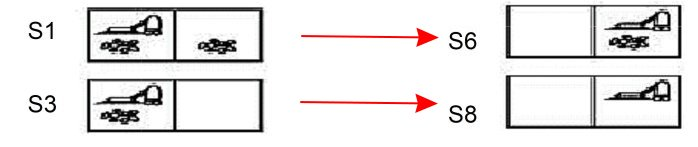
\includegraphics[width=0.8\textwidth]{figures/roomba-zufall.png}
    \caption{Roomba Zufallproblem}
    \label{fig:roomba-zufall}
\end{figure}

\paragraph{4. Explorations-Probleme}

Der L�ser hat keine Kenntnis von der Welt und muss seine Umgebung erkunden, um die m�glichen Zust�nde und die Auswirkungen seiner Aktionen zu erfahren.

Ein gutes Beispiel daf�r ist der Marsrover. Der Rover muss zun�chst Daten sammeln, um seine Umgebung kennenzulernen und eine Karte zu erstellen. Mit dieser Karte kann es dann erfolgreich die Pfadfindung durchf�hren.